\section{一般原理}

\subsection{定义}

\begin{definition}[分治 Divide and Conquer]
    字面上的解释是 ``分而治之'',就是把一个复杂的问题分成两个或更多的相同或相似的子问题,直到最后子问题可以简单的直接求解,原问题的解即子问题的解的合并。
\end{definition}

\subsection{过程}

分治算法的核心思想就是 ``分而治之''。

大概的流程可以分为三步:\textbf{分解 $\to$ 解决(触底) $\to$ 合并(回溯)}。\begin{enumerate}
    \item 分解原问题为结构相同的子问题。
    \item 分解到某个容易求解的边界之后,进行递归求解。
    \item 将子问题的解合并成原问题的解。
\end{enumerate}
分治法能解决的问题一般有如下特征:\begin{itemize}
    \item 该问题的规模缩小到一定的程度就可以容易地解决。
    \item 该问题可以分解为若干个规模较小的相同问题,即该问题具有\textbf{最优子结构性质}。
    \item 利用该问题分解出的子问题的解可以合并为该问题的解。
    \item 该问题所分解出的各个子问题是相互独立的,即子问题之间不包含公共的子问题。
\end{itemize}

如果各子问题是不独立的,则分治法要重复地解公共的子问题,也就做了许多不必要的工作。此时虽然也可用分治法,但一般用\textbf{动态规划}较好。

在用分治法设计算法时,最好使子问题的规模大致相同:即将一个问题分成大小相等的 $k$ 个子问题的处理方法是行之有效的。这种使子问题规模大致相等的做法是出自一种\textbf{平衡(balancing)子问题}的思想,它几乎总是比子问题规模不等的做法要好。

\subsection{递归与分治的区别}

递归是一种编程技巧,一种解决问题的思维方式;分治算法很大程度上是基于递归的,解决更具体问题的算法思想。

\section{问题}

给定一个有 $n$ 个数的无序的数组,查找其中排序好后的第 $k$ 大的元素(排序从1开始)。

比较不同规模下 $n=1000,100000,1000000$ 到 10000000,且 $k$ 取在有序后的头部、中间和尾部时(比如,间隔为 $n/8$ 的方式)各自的时间复杂度,比较相关的差异,画出曲线图。

\section{算法设计}

\subsection{随机选择}

\subsubsection{基本流程}

\begin{algorithm}[htbp]
    \label{alg:quickSelect}
    \SetAlgoLined
    \SetKwInput{KwIn}{输入}
    \SetKwInput{KwOut}{输出}
    \KwIn{数组 $nums$, 左边界 $left$, 右边界 $right$, 第 $k$ 大的元素位置 $k$, 随机数生成器 $gen$}
    \KwOut{第 $k$ 大的元素}
    
    \If{$left == right$}{
        \Return $nums[left]$\;
    }
    
    % 随机选择主元
    $pivotIndex \leftarrow$ 随机整数生成于 $[left, right]$ \;
    $pivot \leftarrow nums[pivotIndex]$\;
    
    % 将主元移到末尾
    交换 $nums[pivotIndex]$ 和 $nums[right]$\;
    
    % 划分操作
    $storeIndex \leftarrow left$\;
    \For{$i \leftarrow left$ \textbf{to} $right - 1$}{
        \If{$nums[i] > pivot$}{ % 查找第 k 大,因此使用 > 符号
            交换 $nums[i]$ 和 $nums[storeIndex]$\;
            $storeIndex \leftarrow storeIndex + 1$\;
        }
    }
    
    % 将主元放到正确的位置
    交换 $nums[storeIndex]$ 和 $nums[right]$\;
    
    % 计算主元位置相对于第 k 大的位置
    $count \leftarrow storeIndex - left + 1$\;
    \If{$count == k$}{
        \Return $nums[storeIndex]$\;
    }
    \ElseIf{$k < count$}{
        \Return \textbf{quickSelect}($nums$, $left$, $storeIndex - 1$, $k$, $gen$)\;
    }
    \Else{
        \Return \textbf{quickSelect}($nums$, $storeIndex + 1$, $right$, $k - count$, $gen$)\;
    }
    
    \caption{基于随机选择方式的分治法查找第 $k$ 大元素}
    \end{algorithm}    
    \begin{description}
        \item[基线情况] 如果当前查找范围内只有一个元素,直接返回该元素。
        \item[随机选择主元] 在当前范围内随机选择一个主元元素,并将其移动到数组的末尾。
        \item[划分操作] 将所有大于主元的元素移动到左侧,记录分割点 \texttt{storeIndex}。
        \item[递归查找] \begin{itemize}
            \item 如果主元的位置正好是第 $k$ 大的位置,返回主元元素。
            \item 如果第 $k$ 大的元素在左侧子数组中,递归查找左侧。
            \item 否则,在右侧子数组中继续查找,并调整 $k$ 的值。
        \end{itemize}
    \end{description}
    算法伪代码如算法~\autoref{alg:quickSelect} 所示。
\subsubsection{复杂度分析}

\textbf{最好情况}:在最好情况下,我们有可能在第一次随机选择主元时,该主元便是我们要寻找的\textbf{第 $k$ 大}的元素,因此只需要一次遍历进行划分,即将剩余的 $n - 1$ 个元素与主元进行一次比较,时间复杂度为 $\Theta(n - 1)$ 即 $\Theta(n)$。

也就是说在最好情况下,\texttt{quickSelect} 的时间复杂度为 $\Theta(n)$

\textbf{最坏情况}:每次选择的主元是当前范围内的\textbf{最大}或\textbf{最小}元素,导致一侧子数组为空或仅含一个元素,另一侧子数组大小为 $n - 1$。

每次划分需要遍历当前数组范围,时间为 $\Theta(n)$,每次仅减去一个元素,递归深度为 $n$。

因此很容易得到,在最坏情况下,\texttt{quickSelect} 的时间复杂度为 $\Theta(n^2)$,值得一提的是,由于我们的主元是随机选择的,因此不存在一个特定的会导致最坏情况发生的输入数据。

\textbf{平均情况}:为了分析 \texttt{quickSelect} 在平均情况下的时间复杂度,也即算法的期望运行时间,我们设该算法在一个含有 $n$ 个元素的输入数组 $A[p\dots r]$ 上的运行时间是一个随机变量,记为 $T(n)$,我们的目的就是求解 $E(T(n))$ 的一个上界。我们设置了 cpp 的随机数生成器 \texttt{std::mt19937} 是等概率分布的,因此任何元素作为主元的概率是相同的。也就是说,对于每一个 $k(1\leq  k \leq  n)$,字数组 $A[p \dots q]$ 有 $k$ 个元素(全部小于或等于主元)的概率是 $1/n$。对所有 $k=1,2,\dots,n$,定义指示器随机变量 $X_k$ 为:\[X_k=I\{\text{字数组 }A[p\dots q] \text{ 正好包含 } k \text{ 个元素}\}\]
然后,假设元素是互异的,我们有:\begin{equation}
    E[X_k]=1/n
    \label{eq:expectation}
\end{equation}
当调用随机数生成器并选择 $A[q]$ 选择主元时,事先并不知道是否会立即得到正确答案而结束,但是可以确定,下一次,要么在子数组 $A[p\dots q-1]$ 上递归,要么在子数组 $A[q+1\dots r]$ 上递归。这取决于第 $i$ 小的元素相对于 $A[q]$ 落在那个位置。显然,我们可以假设 $T(n)$ 是随着 $n$ 单调递增的,因此,通过评估最大可能的输入数据递归调用所需时间,我们可以给出递归调用所需要时间的上界。也就是说,为了得到上界,我们假定第 $i$ 个元素总是在划分中包含较多元素的一边。对一个确定的随机数生成器,指示器随机变量 $X_k$ 恰好在给定的 $k$ 值上取值 1,对其他值都为 0.当 $X_k=1$ 时,我们可能要递归处理的两个字数组的大小分别为 $k-1$ 和 $n-k$。因此我们可以得到递归式:\begin{align*}
    T(n)&\leq \sum_{k=1}^{n}X_{k}\cdot(T(\max(k-1,n-k))+O(n))\\
    &=\sum_{k=1}^{n}X_{k}\cdot T(\max(k-1,n-k))+O(n)
\end{align*}
其中,$O(n)$是遍历划分所需要的时间,是算法运行时间中的非递归部分。两边同时取期望值,得到
\begin{align*}E[T(n)]&\leq E\bigg[\sum_{k=1}^{n}X_{k}\cdot T(\max(k-1,n-k))+O(n)\bigg]\\&=\sum_{k=1}^{n}E[X_{k}\cdot T(\max(k-1,n-k))]+O(n)\quad\text{(期望的线性性质)}\\&=\sum_{k=1}^{n}E[X_{k}]\cdot E[T(\max(k-1,n-k))]+O(n)\quad\text{(期望的乘积性质)}\\&=\sum_{k=1}^{n}\frac{1}{n}\cdot E[T(\max(k-1,n-k))]+O(n)\quad(\text{利用~\autoref{eq:expectation}})\end{align*}
此处显然依赖于 $X_k$ 和 $T(\max(k-1,n-k))$ 是独立的随机变量,我们省略了证明。

下面考虑表达式 $\max(k-1,n-k)$。我们有\[\max(k-1,n-k)=\begin{cases}k-1&\text{若 }k>\lceil n/2\rceil\\n-k&\text{若 }k\leq \lceil n/2\rceil\end{cases}\]
如果$n$是偶数,则从$T(\lceil n/2\rceil)$到$T(n-1)$的每一项在总和中恰好出现两次。如果$n$是奇数,除了$T(\lfloor n/2\rfloor)$出现一次以外,其他这些项也都会出现两次。因此,我们有\[E [T(n)]\leq \frac{2}{n}\sum_{k=\lfloor n/2\rfloor}^{n-1}E [T(k)]+O(n)\]
使用替代法证明$E[T(n)]=O(n)$。假设对于满足这个递归式初始条件的某个常数 $c$,有$E[T(n)]\leq  cn$。假设对小于某个常数的 $n$,有 $T(n)=O(1)$(稍后将用到这个常数)。同时,还要选择一个常数$a$,使得对上式中 $O(n)$ 项所描述的表示划分的函数,对于所有的 $n>0$,有上界 $an$。利用这个归纳假设,可以得到:\begin{align*}
    E[T(n)]& \leq \frac{2}{n}\sum_{k=\lfloor n/2\rfloor}^{n-1}ck+an \\
    &=\frac{2c}{n}\Big(\sum_{k=1}^{n-1}k-\sum_{k=1}^{\lfloor n/2\rfloor-1}k\Big)+an \\
    &=\frac{2c}{n}\Big(\frac{(n-1)n}{2}-\frac{(\lfloor n/2\rfloor-1)\lfloor n/2\rfloor}{2}\Big)+an \\
    &\leq \frac{2c}{n}\Big(\frac{(n-1)n}{2}-\frac{(n/2-2)(n/2-1)}{2}\Big)+an \\
    &=\frac{2c}{n}\Big(\frac{n^{2}-n}{2}-\frac{n^{2}/4-3n/2+2)}{2}\Big)+an \\
    &=\frac{c}{n}\Big(\frac{3n^{2}}{4}+\frac{n}{2}-2\Big)+an \\
    &=c\Big(\frac{3n}{4}+\frac{1}{2}-\frac{2}{n}\Big)+an \\
    &\leq \frac{3cn}4+\frac{c}2+an \\
    &=cn-\left(\frac{cn}4-\frac c2-an\right)
\end{align*}
为了完成证明,还需要说明:对足够大的$n$,最后一个表达式至多是$cn$,等价地,需要证明 $cn/4-c/2-an\geq0$。如果在上式两边同时加$c/2$,并且提取因子$n$,可以得到$n(c/4-a)\geq c/2$。只要我们选择的常数$c$能够满足$c/4-a>0$,即$c> 4a$, 就可以将不等式两边同时除以 $c/ 4- a$,得到\[n\geq\frac{c/2}{c/4-a}=\frac{2c}{c-4a}\]
因此,如果假设对所有$n<2c/(c-4a)$,都有$T(n)=O(1)$,那么就有 $E[T(n)]=O(n)$。我们便可以得出这样的结论:假设所有元素是互异的,在期望线性时间内,我们可以找到任一顺序的数组中第 $k$ 大的元素。也即算法的平均时间复杂度为 $O(n)$。

此外,我们还可以知道,尽管最坏情况下时间复杂度较高,但由于随机选择主元的策略,最坏情况发生的概率极低,对于 $n = 100$,这个概率大约是$2^{n-1}/n!$(每次选择最大或最小,共 $n-1$ 次)即$6.79\times10^{-129}$,已经可以忽略不计,更不用说 $n$ 取更大的情况。在实际应用中,\texttt{quickSelect} 通常表现出线性的时间复杂度,实际上,该方法是一个十分高效的算法。

\textbf{空间复杂度分析}:对于空间复杂度,我们主要关注算法在执行过程中所需的额外内存空间,因此输入数据存储不计入空间复杂度。算法操作的是输入数组 \texttt{nums},但由于操作是原地进行(即在原数组上进行元素交换),因此不需要额外的数组存储空间。由于 \texttt{quickSelect} 是一个递归算法,且由于传递参数时,传递的是数组的引用,因此递归调用的栈空间不会产生对原数组的拷贝,但是算法中使用了少量的辅助变量(如 \texttt{pivotIndex}、\texttt{pivot}、\texttt{storeIndex} 等),这些变量的空间需求与输入规模无关,可以视为常数,由于会有常数的栈空间开销,空间递归深度直接影响算法的空间复杂度。

由前面的分析我们可以知道递归深度,因此很容易可以得出,平均情况下 \texttt{quickSelect} 的空间复杂度为 \( O(\log n) \),最坏情况下的空间复杂度为 \( O(n) \)。

\subsection{确定的线性时间选择}

\subsubsection{基本流程}

\begin{algorithm}[htbp]
    \label{alg:deterministicSelect}
    \SetAlgoLined
    \DontPrintSemicolon
    \SetKwInOut{Input}{输入}
    \SetKwInOut{Output}{输出}
    
    \Input{数组 $nums$, 左边界 $left$, 右边界 $right$, 第 $k$ 大的元素位置 $k$}
    \Output{第 $k$ 大的元素}
    
    \If{$right - left + 1 \leq  5$}{
        \Return \textbf{findMedian}($nums$, $left$, $right$)\;
    }
    
    % 将数组分成每组最多5个元素,找到每组的中位数
    $medians \leftarrow \emptyset$\;
    \For{$i \leftarrow left$ \textbf{to} $right$ \textbf{step} 5}{
        $sub\_right \leftarrow \min(i + 4, right)$\;
        $median \leftarrow$ \textbf{findMedian}($nums$, $i$, $sub\_right$)\;
        $medians.\text{append}(median)$\;
    }
    
    % 递归地找到中位数的中位数
    $medianOfMedians \leftarrow$ \textbf{deterministicSelect}($medians$, $0$, $medians.\text{size()} - 1$, $\lceil \frac{medians.\text{size()}}{2} \rceil$)\;
    
    % 找到中位数的索引
    $pivotIndex \leftarrow$ \textbf{findIndex}($nums$, $left$, $right$, $medianOfMedians$)\;
    
    % 将主元移到末尾
    \textbf{swap}($nums[pivotIndex]$, $nums[right]$)\;
    
    % 划分操作
    $storeIndex \leftarrow left$\;
    \For{$i \leftarrow left$ \textbf{to} $right - 1$}{
        \If{$nums[i] > medianOfMedians$}{ % 查找第 $k$ 大,因此使用 > 符号
            \textbf{swap}($nums[i]$, $nums[storeIndex]$)\;
            $storeIndex \leftarrow storeIndex + 1$\;
        }
    }
    
    % 将主元放到正确的位置
    \textbf{swap}($nums[storeIndex]$, $nums[right]$)\;
    
    % 计算主元位置相对于第 $k$ 大的位置
    $count \leftarrow storeIndex - left + 1$\;
    \If{$count == k$}{
        \Return $nums[storeIndex]$\;
    }
    \ElseIf{$k < count$}{
        \Return \textbf{deterministicSelect}($nums$, $left$, $storeIndex - 1$, $k$)\;
    }
    \Else{
        \Return \textbf{deterministicSelect}($nums$, $storeIndex + 1$, $right$, $k - count$)\;
    }
    
    \caption{基于确定性选择的分治法查找第 $k$ 大元素}
    \end{algorithm}
    \begin{algorithm}[htbp]
        \label{alg:findMedian}
        \SetAlgoLined
        \DontPrintSemicolon
        \SetKwInOut{Input}{输入}
        \SetKwInOut{Output}{输出}
        
        \Input{数组 $nums$, 左边界 $left$, 右边界 $right$}
        \Output{中位数元素}
        % 对子数组 [left, right] 进行排序
        \textbf{Sort}($nums[left \dots right]$)\;
        
        % 计算中位数的索引
        $medianIndex \leftarrow left + \left\lfloor \frac{right - left}{2} \right\rfloor$\;
        
        % 返回中位数
        \Return $nums[medianIndex]$\;
        
        \caption{查找子数组的中位数}
    \end{algorithm}

    \begin{description}
        \item[基线情况] 如果当前查找范围内元素数量不超过5,直接找到并返回中位数。
        \item[分组与中位数收集] 将数组分成每组最多5个元素,分别找到每组的中位数,并将这些中位数存入 \texttt{medians} 数组。
        \item[中位数的中位数]: 递归调用 \texttt{deterministicSelect} 函数,找到 \texttt{medians} 数组的中位数,即 ``中位数的中位数''。
        \item[划分操作] 使用 ``中位数的中位数'' 作为主元,对数组进行划分,使得所有大于主元的元素位于左侧,记录分割点 \texttt{storeIndex}。
        \item[递归查找] \begin{itemize}
            \item 如果主元的位置正好是第 $k$ 大的位置,返回该元素。
            \item 如果第 $k$ 大的元素在左侧子数组中,递归查找左侧子数组。
            \item 否则,在右侧子数组中继续查找,并调整 $k$ 的值。
        \end{itemize}
    \end{description}

    算法伪代码如算法~\autoref{alg:deterministicSelect} 所示,其调用的寻找中位数的子算法如算法~\autoref{alg:findMedian} 所示。
\subsubsection{复杂度分析}

为了分析 \texttt{deterministicSelect} 的时间复杂度,我们首先要确定每次递归的数组的大小。图~\autoref{fig:median} 给出了一个形象的说明。在找出的所有中位数中,至少有一半大于或等于中位数的中位数 $x$(此处我们假假设数组中所有的数都是互异的,所以除了 $x$ 以外的所有元素都大于或小于 $x$。对于不互异的情况,其实也类似,取决于具体实现)。因此,在这 $\lceil n/5 \rceil$ 个组中,除了当 $n$ 不能被 5 整除时产生的所含元素少于 5 的那个组和包含 $x$ 的那个组之外,至少有一半的组中有 3 个元素大于 $x$。不考虑这两个组,大于 $x$ 的元素个数至少为\[3\left(\left\lceil\frac12\left\lceil\frac n5\right\rceil\right\rceil-2\right)\geqslant\frac{3n}{10}-6\]
\begin{figure}[htbp]
    \centering
    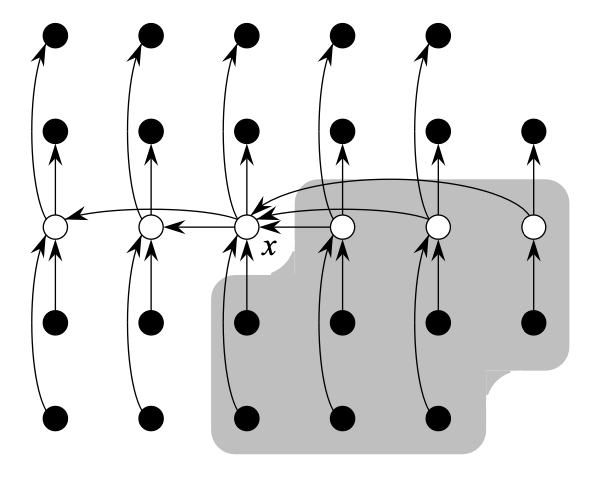
\includegraphics[width=0.6\textwidth]{../figure/analysis.png}
    \caption{算法划分的示意图。所有 $n$ 个元素都由小圈来表示,并且每一组的 5 个元素都在同一列上。其中,每组的中位数用白色圈来表示,而中位数的中位数 $x$ 也被标识出来(当查找偶数个元素的中位数时,使用较小的中位数)。箭头从较大的元素指向较小的元素,从图中可以看出,在$x$的右边,每一个包含5个元素的组中至少有3个元素大于 $x$。在 $x$ 的左边,每一个包含5个元素的组中有3个元素小于$x$。大于$x$的元素的背景以阴影标出。}
    \label{fig:median}
\end{figure}

类似的,至少有 $3n/10-6$个元素小于 $x$。

\textbf{最好情况}:
在最好的情况下,我们可能第一轮选出的中位数的中位数就是我们要寻找的第 $k$ 大的元素。而划分子数组过程并对子数组排序,选出中位数,需要花费 $O(n)$ 的时间,因为对字子数组的排序使用快速排序,时间复杂度为 $O(5\log 5)$,相当于对大小为 $O(1)$ 的集合调用 $O(n)$ 次插入排序。最后的比较划分递归的子数组所需要的时间为 $O(n)$。找到中位数的中位数的递归调用需要的时间为 找到中位数的中位数所需要的时间为 $T(\lceil n/5 \rceil)$。

我们使用替换法来证明这个时间是线性的。更确切地说,我们将要证明对某个适当大的常数 $c$ 和所有的 $n > 0$,有 $T(n) \leq cn$。

首先,我们假设对某个适当大的常数 $c$ 和所有的 $n$,有 $T(n) \leq cn$;如果 $c$ 足够大,这个假设显然成立。同时,还需要挑选一个常数 $a$,使得对于所有的 $n > 0$,之前都提到的 $O(n)$ 项所对应的函数(用来描述算法运行时间中的非递归部分)有上界 $an$。将这个归纳假设代入上述递归式的右边,得到:\begin{align*}
    T(n) &\leq c \lceil n/5 \rceil+ an \\
    &\leq cn/5 + c + an \\
    &= cn + (-4cn/5 + c + an)
\end{align*}

那么,如果下式成立,上式最多是 $cn$:\begin{equation}
    -\frac{4cn}{5} + c + an \leq 0
    \label{eq:inequality_min}
\end{equation}

化简~\autoref{eq:inequality_min},得到 \begin{equation}
    5an \leq (4n - 5)c
    \label{eq:inequality2_min}
\end{equation}

显然我们可以假设,当 $n = 1$ 时,时间复杂度为 $O(1)$,而当 $n \ge 2$ 时,~\autoref{eq:inequality2_min} 等价于不等式 $c \geq 5a(n/(4n-5))$。由于 $n > 1000 > 2$,所以有 $n/(4n-5) \leq 1/3 \leq 1$。因此选择 $c \ge 5a$ 就能够满足~\autoref{eq:inequality_min}。当 $n$ 足够大时,$c$ 的最小值接近于 $5a/4$。

因此在最好情况下,\texttt{deterministicSelect} 算法的时间复杂度为 \( O(n) \)。可以看到,由于多了许多额外的操作,这个方法的常数项显然大于随机选择。

\textbf{最坏情况}:
由之前的分析我们可以知道,至少有 $3n/10-6$个元素小于或大于中位数的中位数 $x$,因此,在最坏情况下,递归调用的子数组最多作用于 $7n/10+6$ 个元素。

由最好情况的分析可以知道,非递归部分的时间复杂度为 $O(n)$。找到中位数的中位数所需要的时间为 $T(\lceil n/5 \rceil)$。但是由于没有找到第 $k$ 大的元素,我们多了在子数组递归所需要的时间,其至多为 $T(7n/10+6)$($T(n)$ 显然可以假设为单调递增的函数)。我们可以得到如下的递归式:\[T(n)\leq T(\lceil n/5 \rceil)+T(7n/10+6)+O(n)\]

同样使用替换法来证明这个时间是线性的。假设有某个适当大的常数 $c$ 和 $a$。将这个归纳假设代入上述递归式的右边,得到:\begin{align*}
    T(n) &\leq c \lceil n/5 \rceil + c(7n/10 + 6) + an \\
    &\leq cn/5 + c + 7cn/10 + 6c + an \\
    &= 9cn/10 + 7c + an \\
    &= cn + (-cn/10 + 7c + an)
\end{align*}

那么,如果下式成立,上式最多是 $cn$:\begin{equation}
    -\frac{cn}{10} + 7c + an \leq 0
    \label{eq:inequality}
\end{equation}

化简~\autoref{eq:inequality},得到 \begin{equation}
    10an \leq (n - 70)c
    \label{eq:inequality2}
\end{equation}

当 $n \geq 70$ 时,~\autoref{eq:inequality2} 等价于不等式 $c \geq 10a(n/(n-70))$。由于在我们的实验中,$n$ 最小为 1000,因此 $n \geq 70$ 的条件是满足的。但是由于递归过程中会出现 $n \leq 70$ 的情况,由于 $n$ 在此时是一个很小的数,我们可以认为当 $n \leq 70$ 时,时间复杂度为 $O(1)$。由于 $n > 1000 > 140$,所以有 $n/(n-70) \leq 2$。因此选择 $c \ge 20a$ 就能够满足~\autoref{eq:inequality}。当 $n$ 足够大时,$c$ 的最小值接近于 $10a$。

因此在最坏情况下,\texttt{deterministicSelect} 算法的时间复杂度仍为\textbf{线性时间} \( O(n) \)。由于``中位数的中位数''策略的使用,避免了极度不均匀的分割,确保算法在任何情况下都能以线性时间运行。

\textbf{平均情况}:由于最坏情况下,时间复杂度为 $O(n)$ 且最优情况下也是 $O(n)$,在求算期望时,我们必然可以通过放缩将不等式放缩到最坏时间复杂度。因此必然可以得出,\texttt{deterministicSelect} 算法的平均时间复杂度为 \( O(n) \)。

\textbf{空间复杂度}:首先,算法将输入数组划分为若干个大小不超过5的小组。对于每个小组,算法需要存储其中位数。由于每个小组包含最多5个元素,找到中位数后,所有中位数将形成一个新的中位数数组。原始数组的大小为 \( n \),则中位数数组的大小为 \( \lceil n/5 \rceil \),这意味着需要 \( O(n) \) 的空间来存储这些中位数。

算法对中位数数组递归地应用相同的选择过程,以找到中位数的中位数作为枢轴。这一递归过程会持续进行,直到基准情况被满足(例如,当中位数数组足够小时)。尽管每一层递归都需要额外的空间来存储中位数数组,但由于每次递归操作处理的数组规模是原始数组的 \( 1/5 \),因此递归的深度为 \( O(\log n) \)。因此,需要花费 \( O(\log n) \) 的空间来存储递归调用的栈空间。此外,对于递归查找大于或小于中间值的中间值元素的情况,可以知道,递归调用的栈深度最多为 $O(\log n)$,因此栈空间的开销也是 $O(\log n)$。

算法在进行划分操作时,是就地进行的,即在原始数组上直接进行元素的交换和重新排列,而不需要额外的辅助数组综上所述,确定性选择算法的主要空间开销来自于存储中位数数组,其空间需求与输入规模 \( n \) 成线性关系。因此,该算法的空间复杂度为线性时间复杂度 \( O(n) \)。

\section{运行结果分析}
\subsection{运行时间比较}
为了保证不受系统等其他因素的干扰,运行时间测量为 10000 次的平均值。
\begin{figure}[H]
    \centering
    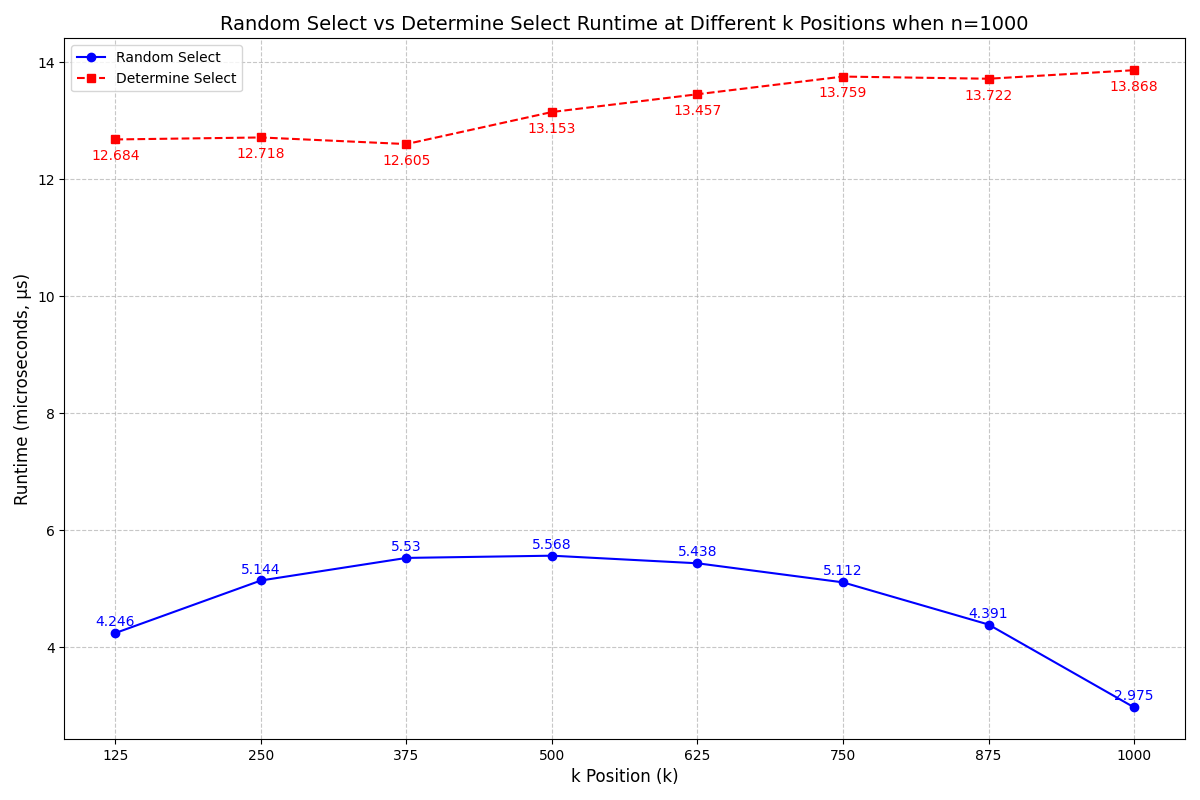
\includegraphics[width=0.7\textwidth]{../figure/1000.png}
    \caption{数组大小为 1000 时的运行时间比较}
\end{figure}
\begin{figure}[H]
    \centering
    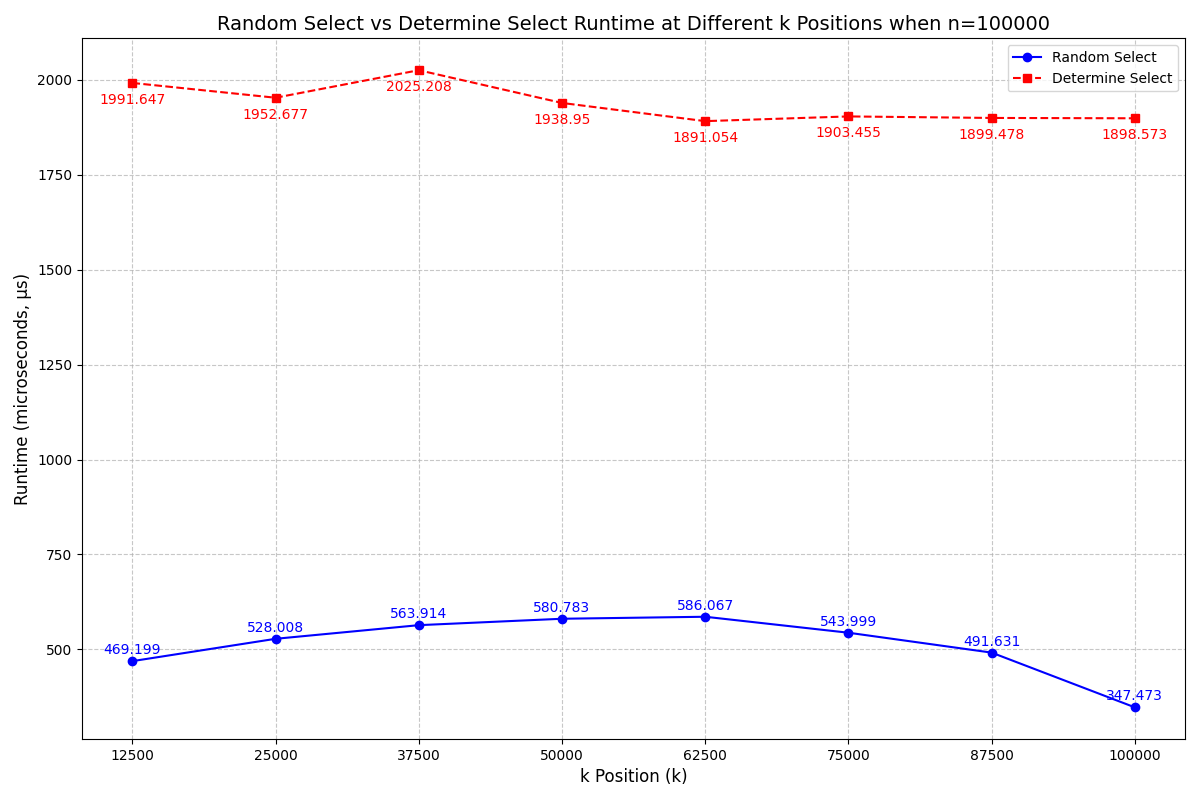
\includegraphics[width=0.7\textwidth]{../figure/100000.png}
    \caption{数组大小为 100000 时的运行时间比较}
\end{figure}
\begin{figure}[H]
    \centering
    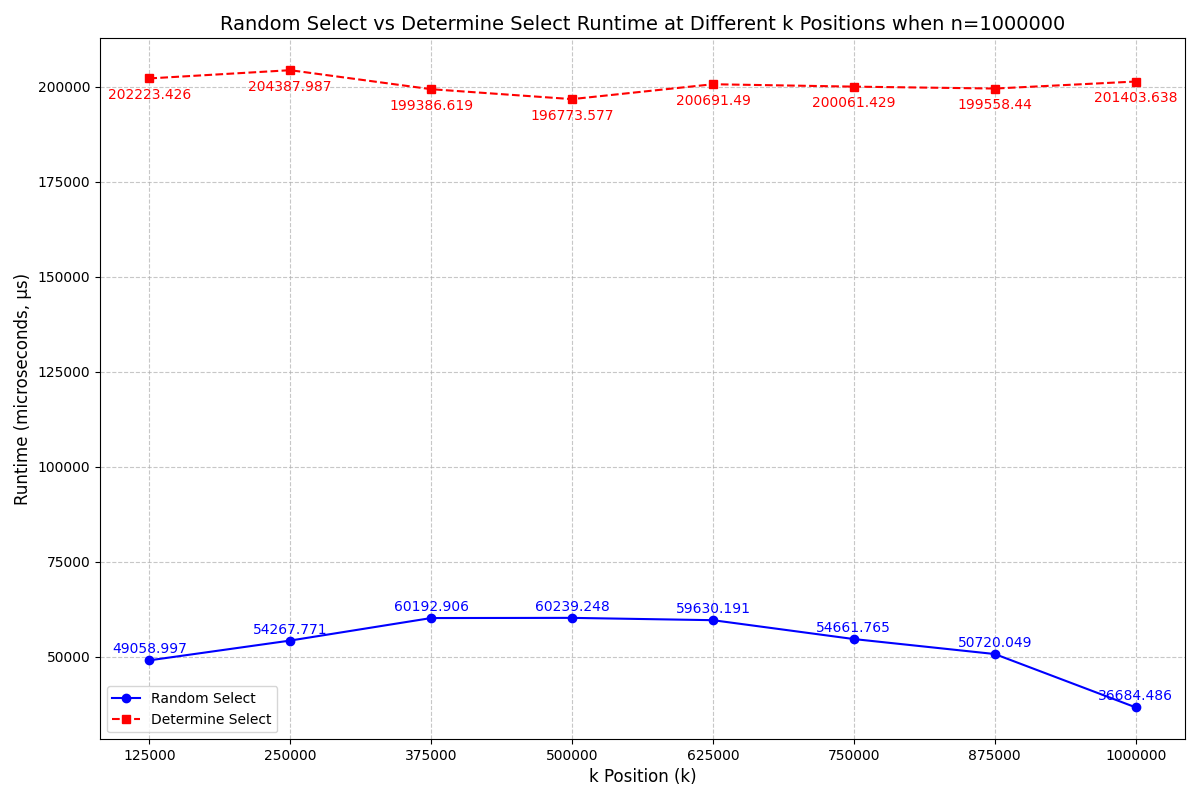
\includegraphics[width=0.7\textwidth]{../figure/1000000.png}
    \caption{数组大小为 1000000 时的运行时间比较}
\end{figure}
\begin{figure}[H]
    \centering
    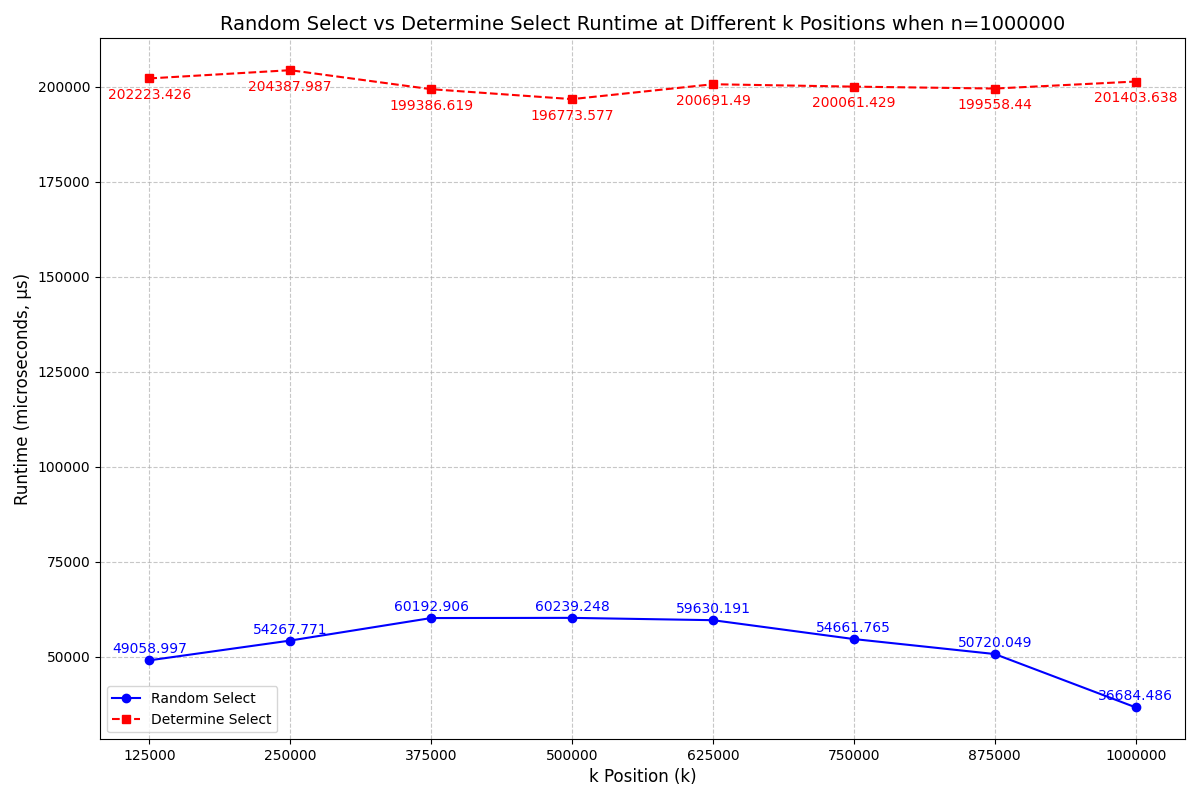
\includegraphics[width=0.7\textwidth]{../figure/10000000.png}
    \caption{数组大小为 10000000 时的运行时间比较}
\end{figure}

可以看到,在 $k$ 依次取在有序后的头部、中间和尾部时,随机选择方法呈现出运行时间先增加后减少的趋势,而确定性选择方法则保持线性稳定上下波动的运行时间。且确定性选择方法的时间一直保持在随机选择方法的 3-4 倍左右。

为了便于比较,我们以数组大小 $n$ 为横坐标,将两种方式放在一起比较,得到如~\autoref{fig:compare_all} 所示的图像。
\begin{figure}[H]
    \centering
    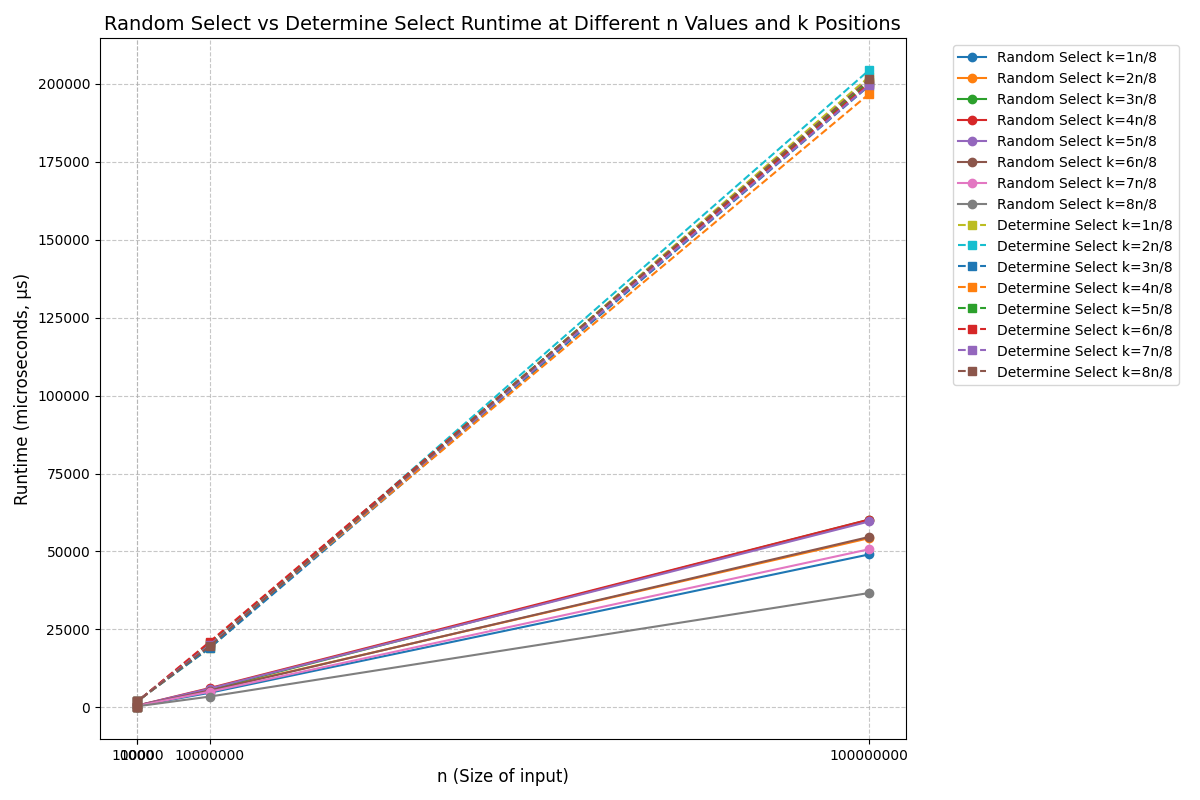
\includegraphics[width=0.65\textwidth]{../figure/compare_all.png}
    \caption{两种选择方法的运行时间比较}
    \label{fig:compare_all}
\end{figure}

上述图像有很明显的 $O(n)$ 的特征,这也反映了两种方法在一般的数据分布中,都是 $O(n)$的,并不会出现随机化选择退化到$O(n^2)$的情况。

\subsection{分析特点比较}
确定性选择算法通过确保每次划分都能有效地缩小搜索范围,保持了线性稳定的运行时间,不受 $k$ 取值位置的影响。而随机选择算法 \texttt{quickSelect} 在不同 $k$ 值下呈现出运行时间先增加后减少的趋势,当 $k$ 取极端值时,所需要的时间更短,当 $k$ 取中间值时,需要的时间更长。

分析其原因,可能是当 $k$ 接近极端值时,无论随机选择选择什么数字作为主元,每次递归都能显著减少剩余需要处理的元素数量,而寻找中位数时,尽管每次也能减少,但需要的递归次数更多,导致总体运行时间更长。但是可以见到,上述变化并不明显,这说明 $k$ 的影响并不大。

从上面的对比实验也可以看到,虽然在最坏情况下,确定性选择的时间复杂度比随机选择要好,但是在实际情况中,结果发现,随机选择的时间明显比确定选择要短。
\begin{itemize}
    \item \textbf{算法常数因子的影响}:确定性选择算法通常将数组分成固定大小(本次实验是5)的组,并对每组进行排序以找到中位数。这一过程涉及大量的交换和比较操作,尤其是在处理大规模数据时,分组和排序的开销显著。此外,还需要递归地在中位数数组中寻找中位数的中位数,这进一步增加了递归调用的开销。而随机化选择只需选择一个随机主元,并进行一次简单的划分操作。相比于确定性选择算法,随机化选择的划分过程更为直接和高效,涉及的操作更少。
    \item \textbf{缓存友好性和内存访问模式}:确定性选择算法在分组和排序过程中,会频繁地跳跃访问数组元素,这种不连续的内存访问模式会导致缓存未命中率增加,从而降低性能。随机化选择的划分操作通常在数组中进行顺序扫描和交换,这种连续的内存访问模式更符合现代处理器的缓存机制,能够更好地利用缓存,提升运行效率。
\end{itemize}
因此,在实际应用中,尤其是对于大多数数据分布情况,随机化选择算法由于其较低的常数因子、更好的缓存友好性和更简洁的实现,通常表现得更快,尽管它在最坏情况下可能退化为 $O(n)$ 的时间复杂度。不过,最坏情况发生的概率极低,尤其是在随机化策略有效的情况下,使得随机化选择成为实际中更为常用和高效的选择算法。

\subsection{执行多次查找后运行的变化}

\subsubsection{随机选择}

首先对随机选择进行了测试,选取数组大小为 1000000 的不同 $k$ 取值进行测试,每个 $k$ 执行 10000 次,结果如~\autoref{fig:random_continue} 所示。\begin{figure}[htbp]
    \centering
    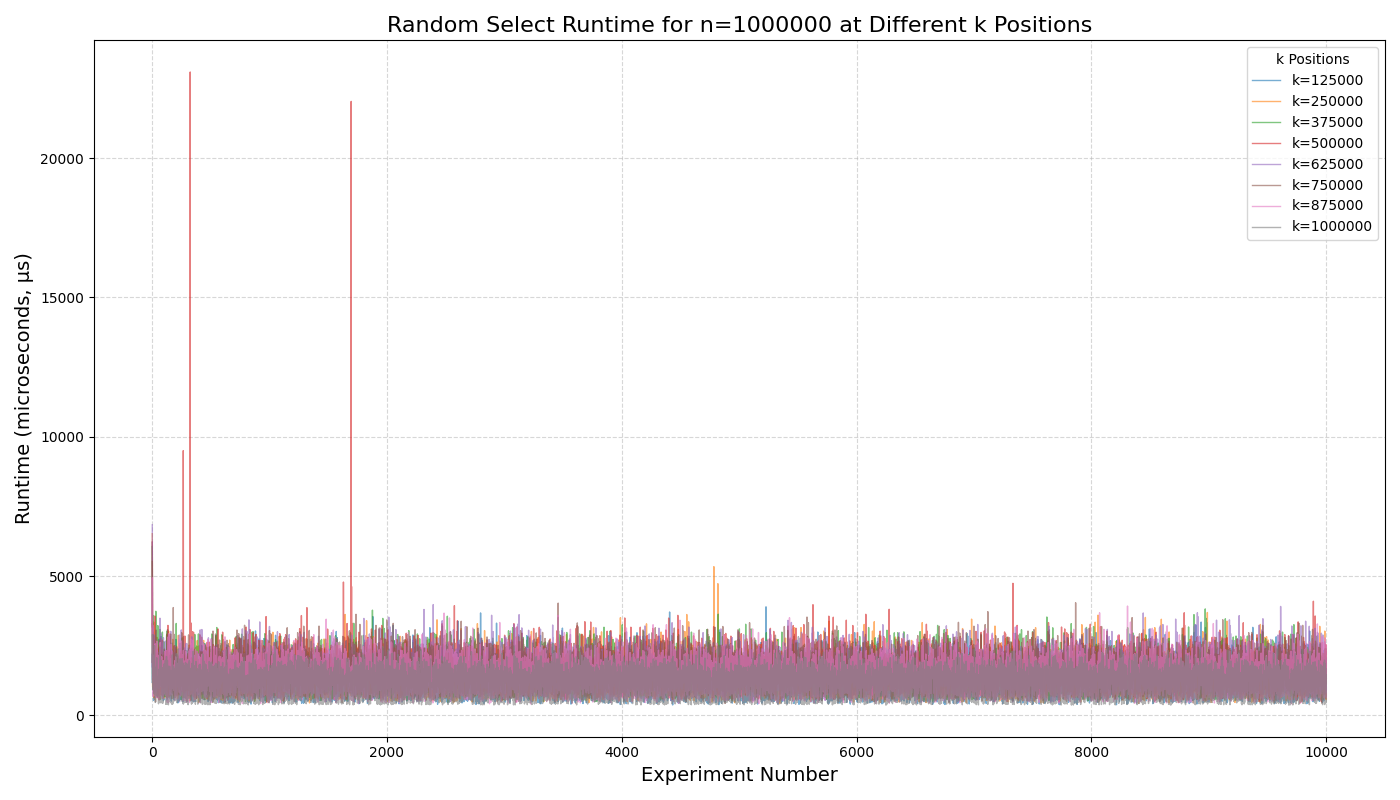
\includegraphics[width=0.7\textwidth]{../figure/random_continue.png}
    \caption{随机选择连续执行 10000 次查找运行时间}
    \label{fig:random_continue}
\end{figure}

可以看到,执行多次查找后,随机选择方法的运行时间并没有明显降低。依然是处于明显波动的状态。原因在于随机选择通选择主元是随机的,这种随机性使得即使数组部分有序,主元选择仍然可能导致不平衡的划分。其次,数组的部分有序性可能不足以显著减少比较和交换操作的数量,因为随机选择的核心操作仍然需要遍历整个数组并进行划分,即使某些区域已经有序,这些局部有序性对全局操作的优化效果有限。

此外可以看到图中存在明显高于其他值的特异值,这反映了随机选择的缺点,即在最坏情况下时间复杂度可能到达 $O(n^2)$,虽然发生最坏情况不太可能,但在 10000 次重复实验中,但是发生较坏的情况是有可能的。

考虑到异常值可能会影响大部分数值情况下的规律判断,选择用四分位数距离($IQR$)利用数据的第25百分位数($Q_1$)和第75百分位数($Q_3$),定义异常值为低于$Q_1 - 1.5 * IQR$或高于$Q_3 + 1.5 * IQR$的值对数据进行了清洗,该方法对数据的分布不做假设,相较于其他方法如 Z-Score 更加稳健。清洗后的时间变化如~\autoref{fig:random_continue_clean}。
\begin{figure}[htbp]
    \centering
    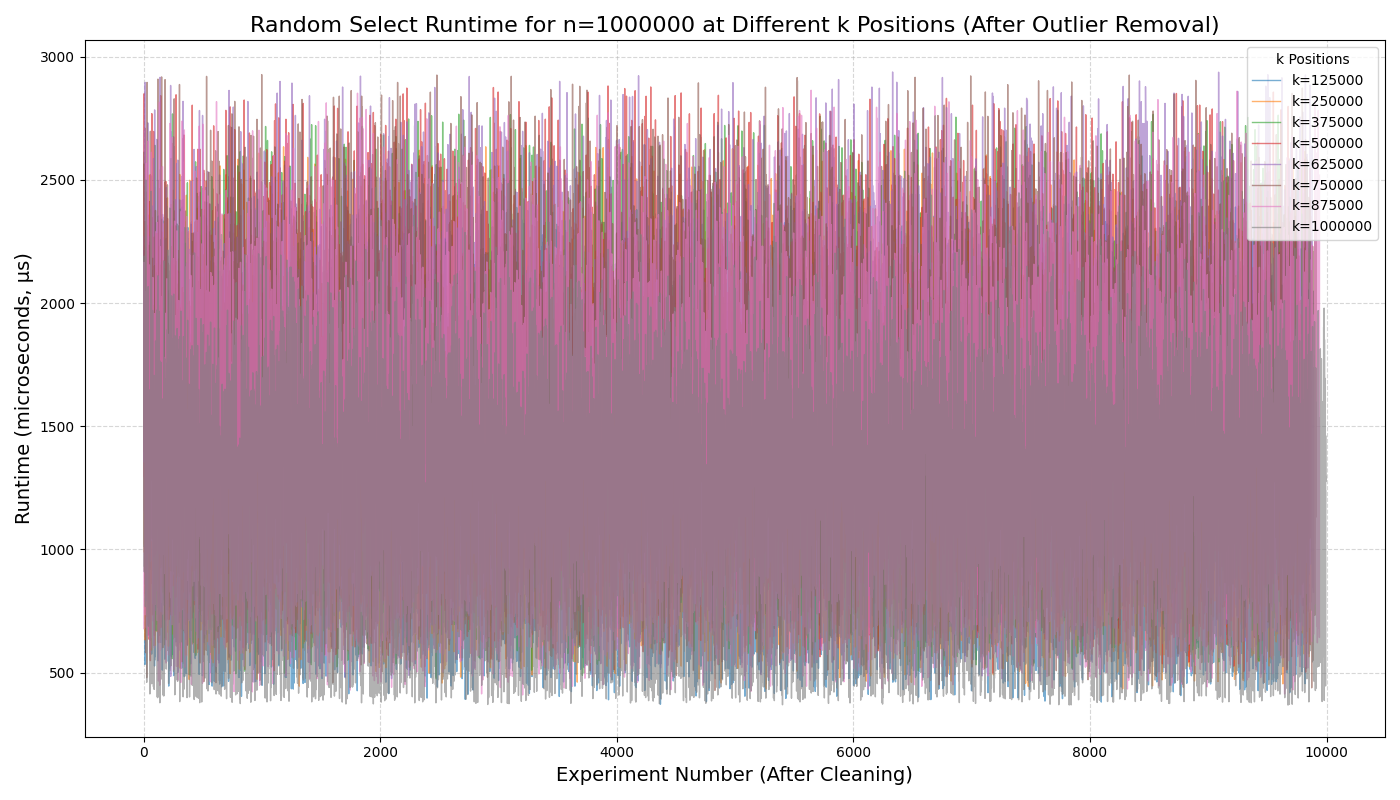
\includegraphics[width=0.7\textwidth]{../figure/random_continue_clean.png}
    \caption{清洗异常值后随机选择运行时间比较}
    \label{fig:random_continue_clean}
\end{figure}

可以看到,仍然没有明显的下降趋势。

\subsubsection{确定性选择}
随后对确定性选择进行了测试。实验次配置保持不变,实验结果如~\autoref{fig:determine_continue} 所示。\begin{figure}
    \centering
    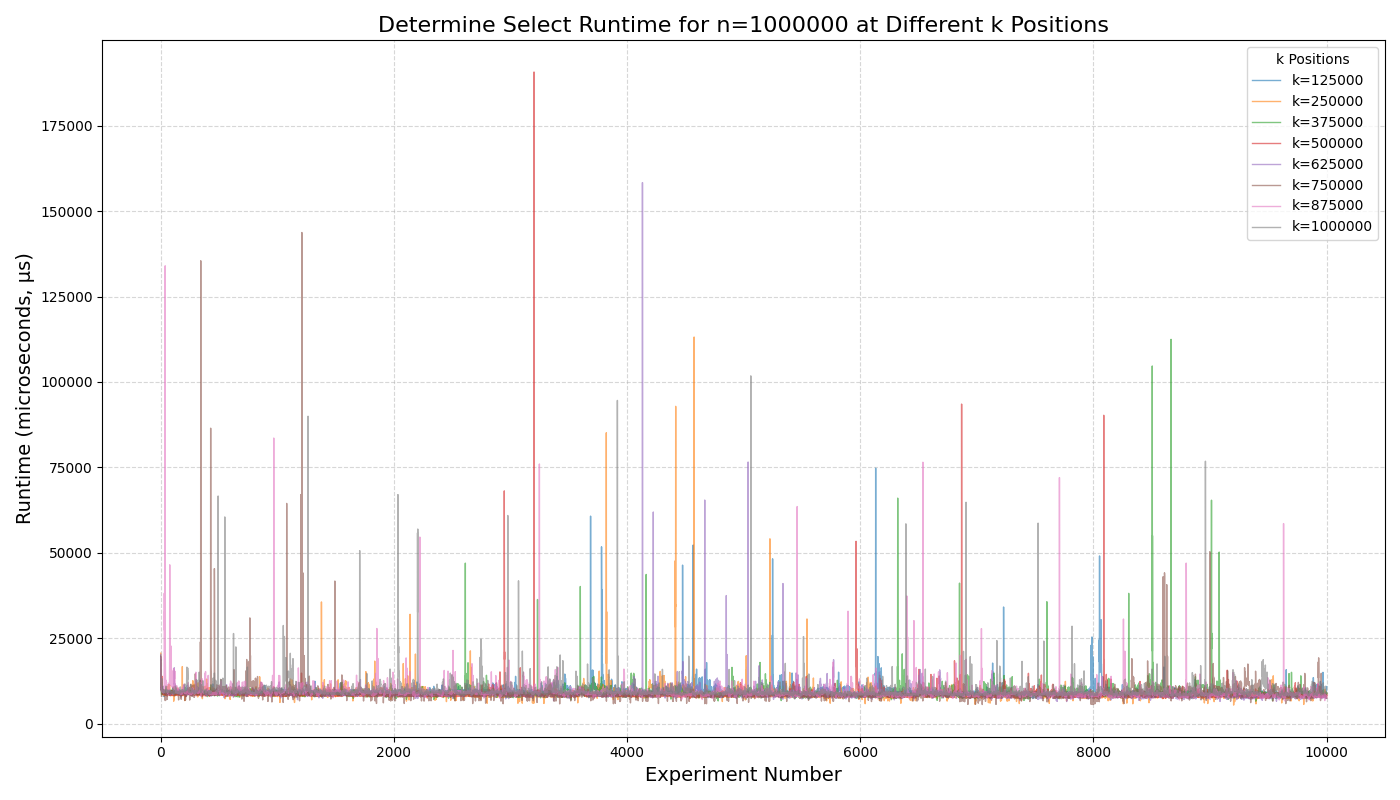
\includegraphics[width=0.7\textwidth]{../figure/determine_continue.png}
    \caption{确定性选择连续执行 10000 次查找运行时间}
    \label{fig:determine_continue}
\end{figure}

可以看到仍然存在特异值,但与随机选择相比,确定性选择的特异值相差没那么大,而且特异值的产生可能是受到实验环境的影响。采用相同的方法去掉特异值后如~\autoref{fig:determine_continue_clean} 所示:
\begin{figure}[htbp]
    \centering
    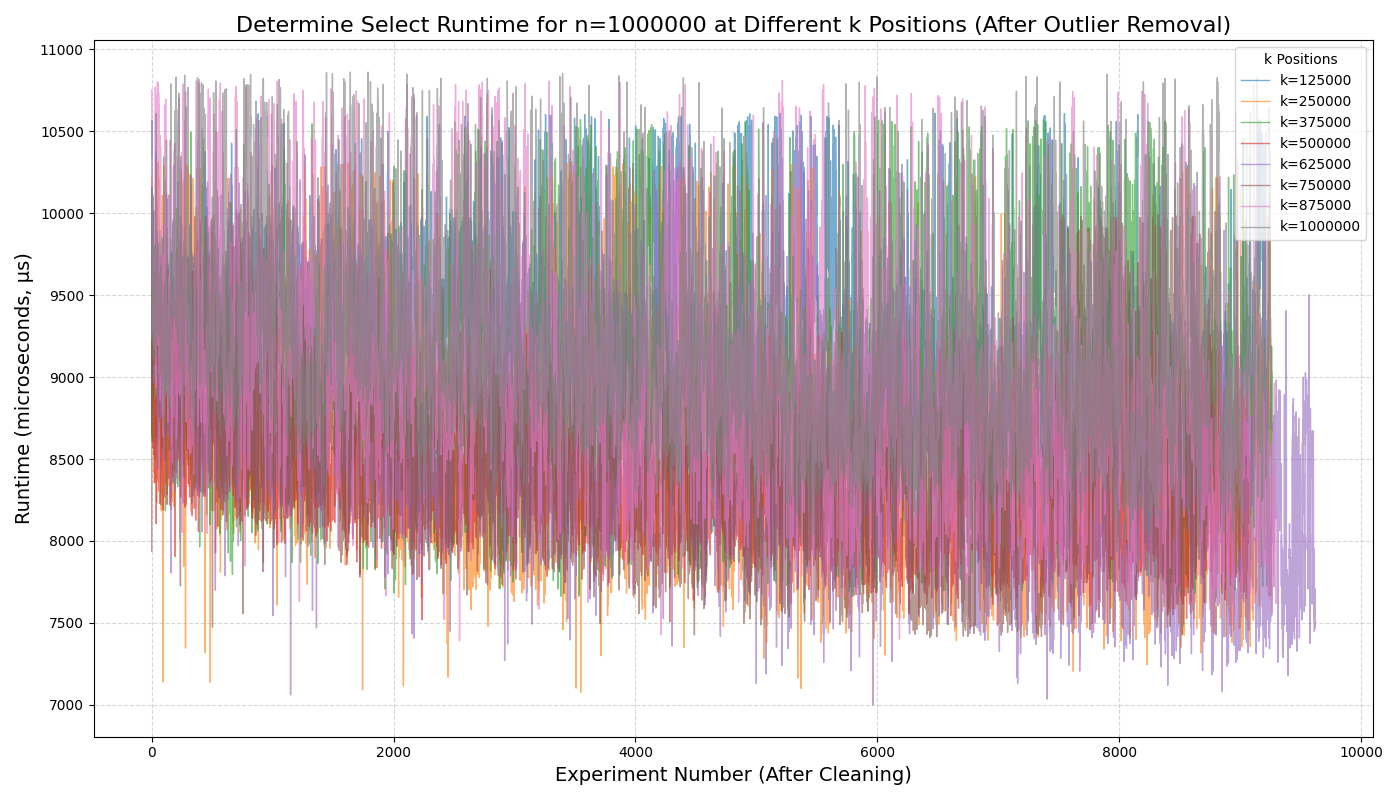
\includegraphics[width=0.7\textwidth]{../figure/determine_continue_clean.png}
    \caption{清洗异常值后确定性选择运行时间比较}
    \label{fig:determine_continue_clean}
\end{figure}

可以看到随着反复查找次数的增加,确定性选择的时间存在着波动中降低的趋势。但是通过分析可以知道,我们使用``中位数的中位数''方法选择主元,即使数据是有序的,算法仍会分组并计算每组的中位数,再从这些中位数中递归找到``中位数的中位数''作为主元,即算法不依赖数据本身的有序性,因此,数据的初始有序性不会显著影响这一过程的时间复杂度和流程。

但是从结果分析,原因可能在于在有序数据中,划分操作变得更加顺滑,因为当数据接近有序时,划划分域时不需要大量的数据移动。现代计算机的缓存机制对访问连续内存块的数据优化较好,因此当数据接近有序时,划分时访问的内存位置更加一致,缓存命中率提升,导致执行时间减少。此外,数据的有序性会使得每次选择的主元 ``中位数的中位数'' 能够将数组近乎均匀地分割为两部分,即每次分割后,左右子数组的大小大致相等(接近 $n/2$),接近算法的最好情况。

此外,\texttt{findMedian} 函数中的排序操作(\texttt{std::sort})会受数据有序性的影响。对于完全有序的数据,排序可能更快。然而,这种排序仅用于小的子数组(每组最多5个元素),这对整体复杂度的影响非常有限。因此,对整体的效率有待考究。

\subsubsection{进一步探究}

为了探究有序数据是否会对确定性选择的运行时间产生影响,我们将之前产生的数组大小 $n$为 1000000 的随机数字排序成有序数据后,对 $k = n / 2$ 的确定性选择进行了对比测试,结果如~\autoref{fig:sorted} 所示。
\begin{figure}[htbp]
    \centering
    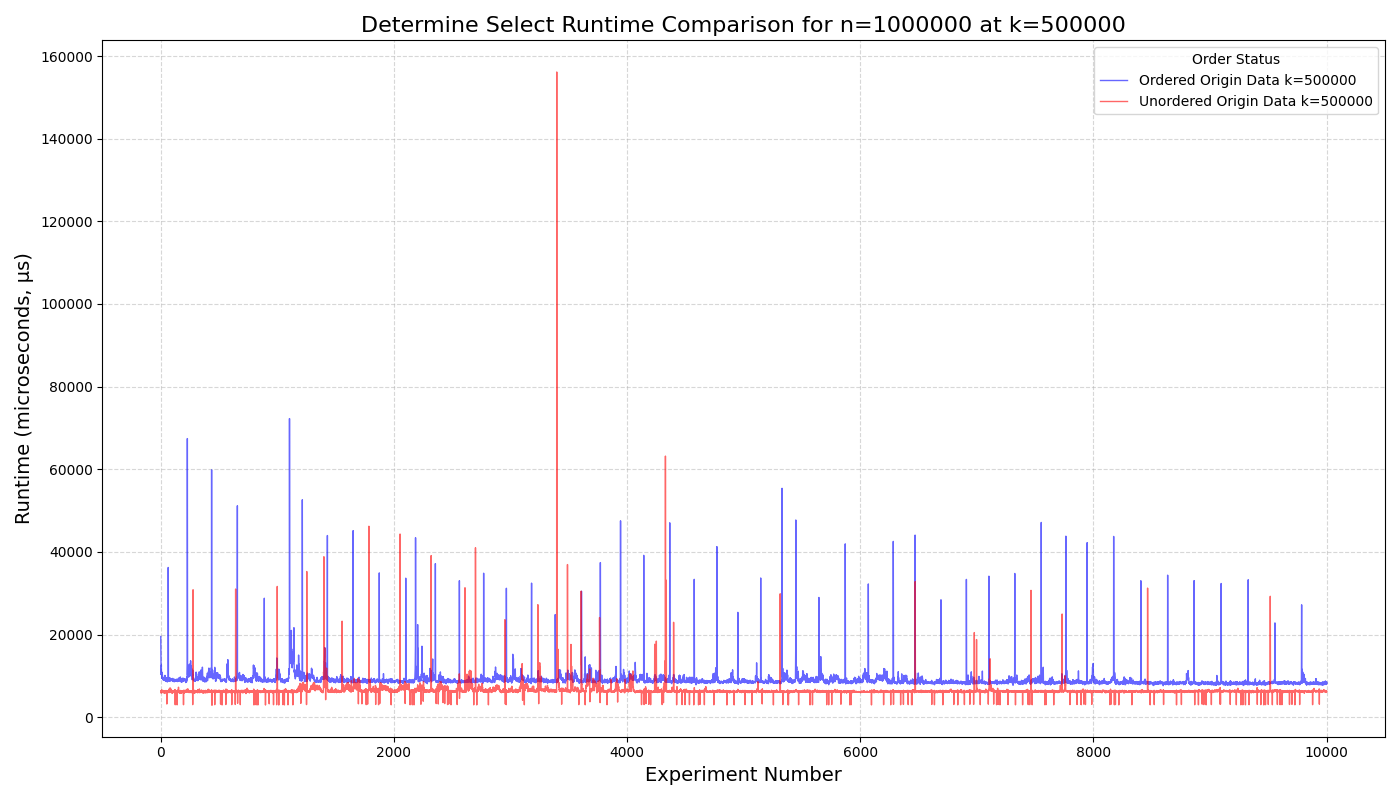
\includegraphics[width=0.7\textwidth]{../figure/determine_continue_order_vs_unorder.png}
    \caption{有序与无序数据的确定性选择运行时间对比}
    \label{fig:sorted}
\end{figure}

为了便于观察,数据清洗后的结果如~\autoref{fig:sorted_clean} 所示。
\begin{figure}[htbp]
    \centering
    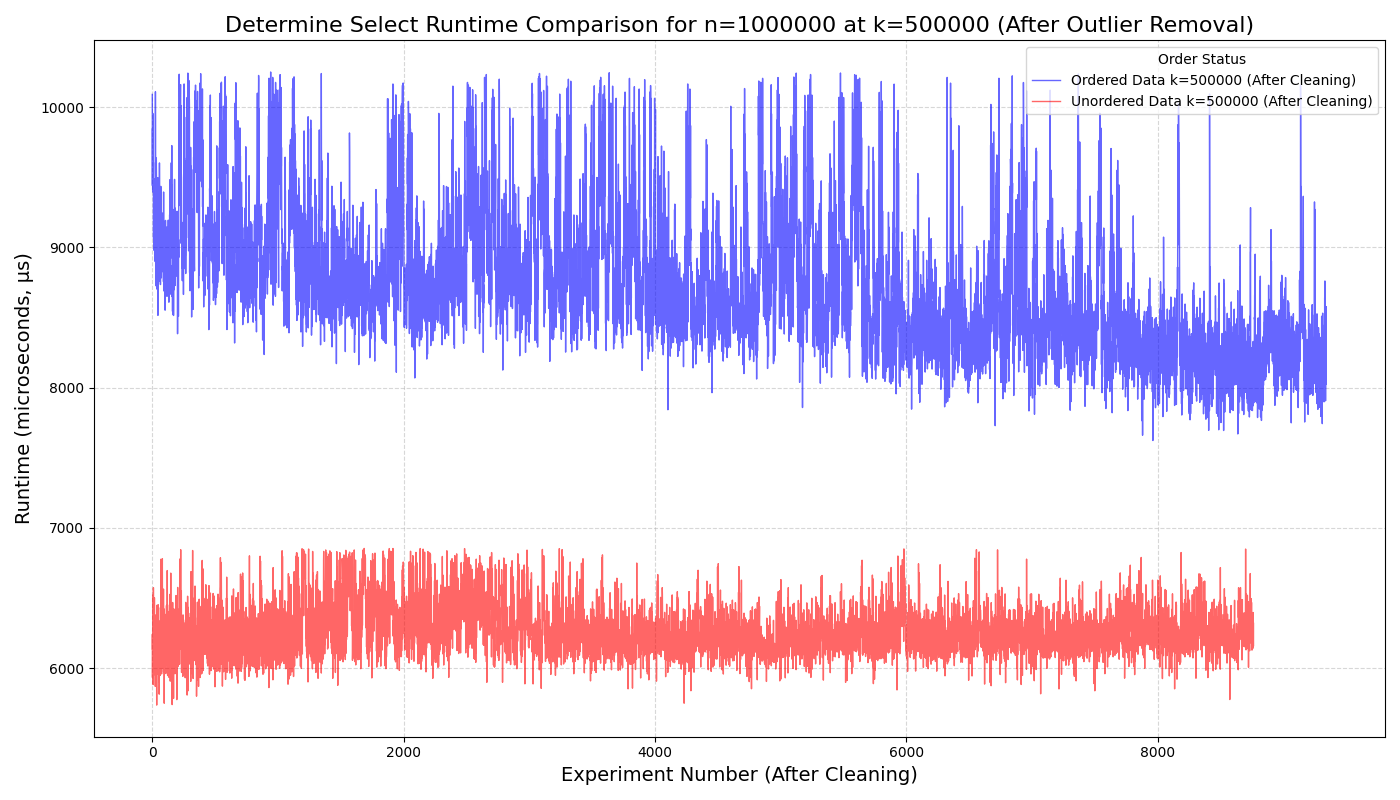
\includegraphics[width=0.7\textwidth]{../figure/determine_continue_order_vs_unorder_cleaned.png}
    \caption{清洗异常值后有序与无序数据的确定性选择运行时间对比}
    \label{fig:sorted_clean}
\end{figure}

可以直观看到,有序数据会对确定性选择的运行时间产生积极影响。有序数据的确定性选择运行时间明显低于无序数据,且有序数据的运行时间更加稳定,波动较小。更加验证了我们的猜想。
\section{算法改进}

\subsection{对确定性选择方法的改进}

由于实验结果表明,确定性选择方法的时间复杂度常数项较大,性能还值得改进。在实际应用中,我们可以考虑以下几种改进方法来减少常数大小:\begin{itemize}
    \item \textbf{减少 \texttt{findMedian} 中的排序开销}:目前的 \texttt{findMedian} 函数对每组的元素进行完全排序,这在最坏情况下是 $O(5 \log 5)$ ,尽管5是常数。实际上,我们只需要找到中位数,而不必对整个数组排序,可以使用选择算法来找出中位数,而不是完全排序。
    \item \textbf{减少对主元元素的查找开销}:目前代码通过 \texttt{std::find} 查找 \texttt{medianOfMedians} 的位置,这是线性时间操作。在划分操作中,可以结合划分和查找来减少一次遍历。通过使用 \cppinline{partitionAroundPivot} 在划分的过程中查找并移动主元,避免二次遍历。
    \item \textbf{递归优化}:通过循环替代递归,减少递归深度,从而提升性能。
\end{itemize}

其算法的逻辑还是与之前类似,我们在数据量 $n$ 为 1000000 的情况下进行了测试,结果如~\autoref{fig:improve} 所示。为了保证不受系统等其他因素的干扰,我们没有采用之前改进前的测试数据,而是同时再次进行测试。
\begin{figure}[htbp]
    \centering
    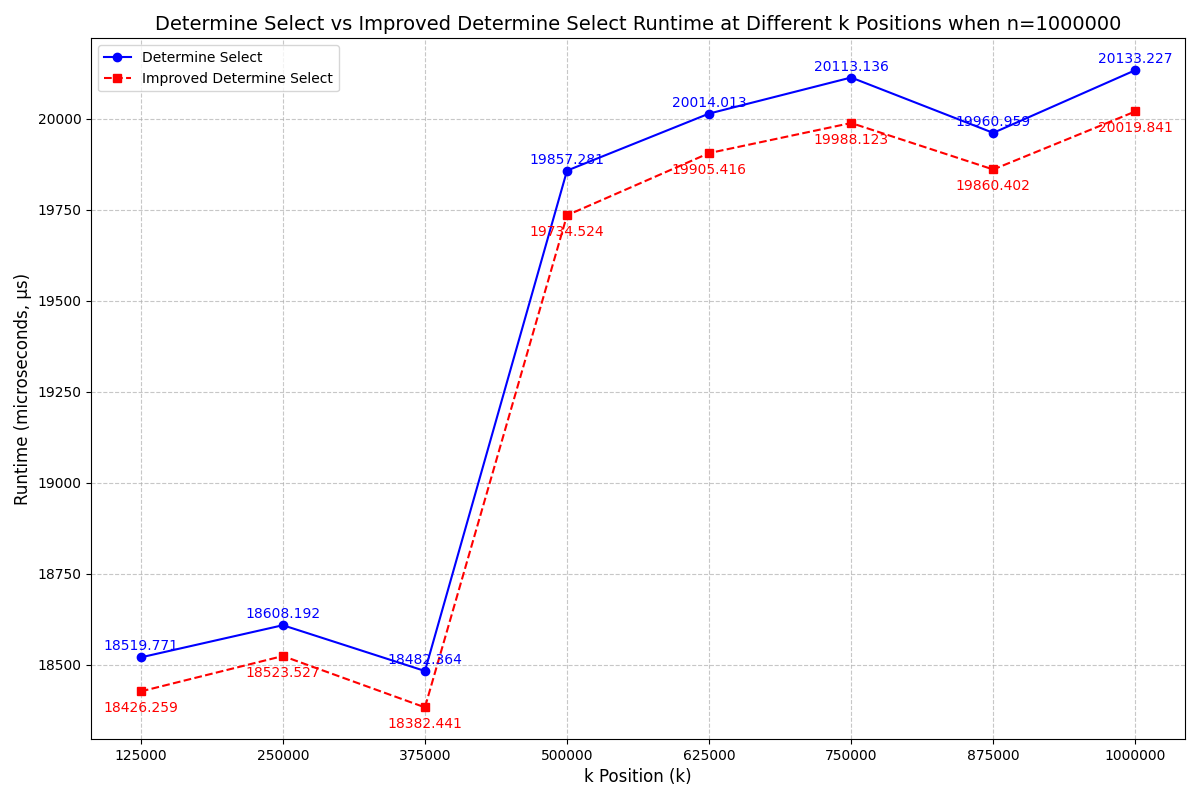
\includegraphics[width=0.7\textwidth]{../figure/determine_compare_1000000.png}
    \caption{改进前后的确定性选择运行时间对比}
    \label{fig:improve}
\end{figure}

可以发现提升了约 120 us。这说明我们的改进方法是有效的,可以减少确定性选择方法的常数项开销,提升算法性能。

\subsection{未完成的探究}

对于确定性时间分组大小的选择,在实验中,我们选择了分组大小为 5,这是一个经验值。在实际应用中,分组大小的选择可能会影响算法的性能。较小的分组大小可能会导致更多的分组和排序操作,增加额外开销;较大的分组大小可能会导致中位数的估计不准确,影响主元的选择。因此,如何选择合适的分组大小是一个值得研究的问题。

此外,数据有序性对确定性选择的运行时间影响也可能与分组大小有关。二者之间的关系也值得深入探究。但是由于时间关系,上述研究没有完成。

\section{总结}

这个实验让我对分治算法有了更深的理解,特别是在选择第 $k$ 大元素的场景下。通过设计和比较随机选择和确定性选择的方法,我体会到了算法效率、理论保证和实际应用之间的微妙平衡。

虽然确定性选择算法通过中位数的中位数策略确保了最坏情况下的线性时间复杂度,但实验中也暴露了其操作复杂度高、常数因子较大的问题。虽然理论上的保证看起来很理想,但在实际中往往需要牺牲简单性和实用性。相比之下,随机选择算法虽然最坏情况下的复杂度可能是二次的,但在实际应用中,尤其是对于典型的数据分布,其表现通常非常好。这让我明白了一个关键的道理:实际效率往往比最坏情况的理论保证更重要,特别是当随机化方法可以有效避免极端情况时。

另一个重要的收获是数据特性对算法性能的影响。当数据有序或无序时,两种方法的表现会有所不同,这让我感到很有趣,并对其展开了深入研究。尤其是在有序数据上,确定性方法的性能有所提升,这表明即使是确定性算法,也可以从输入数据的特性中获益,这和我最初认为其性能不受输入顺序影响的预期有些不同。

此外,这次实验让我更加认识到实现细节的重要性。像如何查找中位数、如何管理主元元素等小的实现选择,都会显著影响算法的性能。这让我更加明白,算法设计不仅是选择什么算法,更重要的是如何去实现它,这直接影响它的效果。

总的来说,这次实验让我意识到,从理论到实践的过程是复杂且充满权衡的。它加深了我对算法思想在面对真实数据和性能限制时如何演变的理解。这次练习在数学严谨性与实践适应性之间找到了平衡,也让我在未来的工作中对算法选择有了更多思考和信心。

\appendix

\section{关键源码}

本试验源代码已经开源到 GitHub。

地址为 \url{https://github.com/Word2VecT/BUPT-Algorithm-Design-and-Analysis-Lab}。

\subsection{随机选择算法}

\begin{cppcode}
// 快速选择算法:查找第 k 大的元素(k 从 1 开始)
int quickSelect(std::vector<int>& nums, int left, int right, int k, std::mt19937& gen) // NOLINT
{
    if (left == right) {
        return nums[left];
    }

    // 随机选择主元
    std::uniform_int_distribution<> dis(left, right);
    int pivotIndex = dis(gen);
    int pivot = nums[pivotIndex];

    // 移动主元到末尾
    std::swap(nums[pivotIndex], nums[right]);

    // 划分
    int storeIndex = left;
    for (int i = left; i < right; ++i) {
        if (nums[i] > pivot) { // 查找第 k 大,因此使用 > 符号
            std::swap(nums[i], nums[storeIndex]);
            storeIndex++;
        }
    }
    // 将主元放到正确的位置
    std::swap(nums[storeIndex], nums[right]);

    // 计算主元位置相对于第 k 大的位置
    int count = storeIndex - left + 1;
    if (count == k) {
        return nums[storeIndex];
    }
    if (k < count) {
        return quickSelect(nums, left, storeIndex - 1, k, gen);
    }
    return quickSelect(nums, storeIndex + 1, right, k - count, gen);
}
\end{cppcode}

\subsection{确定性选择算法}
\begin{cppcode}
// 辅助函数:找到数组的中位数
int findMedian(std::vector<int>& nums, int left, int right) {
    std::sort(nums.begin() + left, nums.begin() + right + 1);
    return nums[left + (right - left) / 2];
}
// 中位数中位数算法:确定性的线性时间选择算法
int deterministicSelect(std::vector<int>& nums, int left, int right, int k) { //NOLINT
    // 如果数组足够小,直接返回中位数
    if (right - left + 1 <= groupSize) {
        return findMedian(nums, left, right);
    }

    // 将数组分成每组最多5个元素,找到每组的中位数
    std::vector<int> medians;
    for (int i = left; i <= right; i += groupSize) {
        int sub_right = std::min(i + 4, right);
        medians.push_back(findMedian(nums, i, sub_right));
    }

    // 递归地找到中位数的中位数
    int medianOfMedians = deterministicSelect(medians, 0, static_cast<int>(medians.size()) - 1, static_cast<int>(medians.size()) / 2);

    // 找到中位数中位数的位置
    std::vector<int>::difference_type pivotIndex = std::distance(nums.begin(), std::find(nums.begin() + left, nums.begin() + right + 1, medianOfMedians));

    // 移动主元到末尾
    std::swap(nums[pivotIndex], nums[right]);

    // 划分
    int storeIndex = left;
    for (int i = left; i < right; ++i) {
        if (nums[i] > medianOfMedians) { // 查找第 k 大,因此使用 > 符号
            std::swap(nums[i], nums[storeIndex]);
            storeIndex++;
        }
    }
    // 将主元放到正确的位置
    std::swap(nums[storeIndex], nums[right]);

    // 计算主元位置相对于第 k 大的位置
    int count = storeIndex - left + 1;
    if (count == k) {
        return nums[storeIndex];
    }
    if (k < count) {
        return deterministicSelect(nums, left, storeIndex - 1, k);
    }
    return deterministicSelect(nums, storeIndex + 1, right, k - count);
}
\end{cppcode}

\subsection{改进后的确定性选择算法}
\begin{cppcode}
// 辅助函数:找到数组的中位数
int findMedian(std::vector<int>& nums, int left, int right) {
    std::sort(nums.begin() + left, nums.begin() + right + 1);
    return nums[left + (right - left) / 2];
}

// 中位数中位数算法:确定性的线性时间选择算法
int deterministicSelect(std::vector<int>& nums, int left, int right, int k) { //NOLINT
    // 如果数组足够小,直接返回中位数
    if (right - left + 1 <= groupSize) {
        return findMedian(nums, left, right);
    }

    // 将数组分成每组最多5个元素,找到每组的中位数
    std::vector<int> medians;
    for (int i = left; i <= right; i += groupSize) {
        int sub_right = std::min(i + 4, right);
        medians.push_back(findMedian(nums, i, sub_right));
    }

    // 递归地找到中位数的中位数
    int medianOfMedians = deterministicSelect(medians, 0, static_cast<int>(medians.size()) - 1, static_cast<int>(medians.size()) / 2);

    // 找到中位数中位数的位置
    std::vector<int>::difference_type pivotIndex = std::distance(nums.begin(), std::find(nums.begin() + left, nums.begin() + right + 1, medianOfMedians));

    // 移动主元到末尾
    std::swap(nums[pivotIndex], nums[right]);

    // 划分
    int storeIndex = left;
    for (int i = left; i < right; ++i) {
        if (nums[i] > medianOfMedians) { // 查找第 k 大,因此使用 > 符号
            std::swap(nums[i], nums[storeIndex]);
            storeIndex++;
        }
    }
    // 将主元放到正确的位置
    std::swap(nums[storeIndex], nums[right]);

    // 计算主元位置相对于第 k 大的位置
    int count = storeIndex - left + 1;
    if (count == k) {
        return nums[storeIndex];
    }
    if (k < count) {
        return deterministicSelect(nums, left, storeIndex - 1, k);
    }
    return deterministicSelect(nums, storeIndex + 1, right, k - count);
}
\end{cppcode}